\documentclass[]{ctexbook}
\usepackage{lmodern}
\usepackage{amssymb,amsmath}
\usepackage{ifxetex,ifluatex}
\usepackage{fixltx2e} % provides \textsubscript
\ifnum 0\ifxetex 1\fi\ifluatex 1\fi=0 % if pdftex
  \usepackage[T1]{fontenc}
  \usepackage[utf8]{inputenc}
\else % if luatex or xelatex
  \ifxetex
    \usepackage{xltxtra,xunicode}
  \else
    \usepackage{fontspec}
  \fi
  \defaultfontfeatures{Ligatures=TeX,Scale=MatchLowercase}
\fi
% use upquote if available, for straight quotes in verbatim environments
\IfFileExists{upquote.sty}{\usepackage{upquote}}{}
% use microtype if available
\IfFileExists{microtype.sty}{%
\usepackage{microtype}
\UseMicrotypeSet[protrusion]{basicmath} % disable protrusion for tt fonts
}{}
\usepackage[b5paper,tmargin=2.5cm,bmargin=2.5cm,lmargin=3.5cm,rmargin=2.5cm]{geometry}
\usepackage[unicode=true]{hyperref}
\PassOptionsToPackage{usenames,dvipsnames}{color} % color is loaded by hyperref
\hypersetup{
            pdftitle={醫學統計學},
            pdfauthor={王 超辰 Chaochen Wang},
            colorlinks=true,
            linkcolor=Maroon,
            citecolor=Blue,
            urlcolor=Blue,
            breaklinks=true}
\urlstyle{same}  % don't use monospace font for urls
\usepackage{natbib}
\bibliographystyle{apalike}
\usepackage{color}
\usepackage{fancyvrb}
\newcommand{\VerbBar}{|}
\newcommand{\VERB}{\Verb[commandchars=\\\{\}]}
\DefineVerbatimEnvironment{Highlighting}{Verbatim}{commandchars=\\\{\}}
% Add ',fontsize=\small' for more characters per line
\usepackage{framed}
\definecolor{shadecolor}{RGB}{248,248,248}
\newenvironment{Shaded}{\begin{snugshade}}{\end{snugshade}}
\newcommand{\KeywordTok}[1]{\textcolor[rgb]{0.13,0.29,0.53}{\textbf{#1}}}
\newcommand{\DataTypeTok}[1]{\textcolor[rgb]{0.13,0.29,0.53}{#1}}
\newcommand{\DecValTok}[1]{\textcolor[rgb]{0.00,0.00,0.81}{#1}}
\newcommand{\BaseNTok}[1]{\textcolor[rgb]{0.00,0.00,0.81}{#1}}
\newcommand{\FloatTok}[1]{\textcolor[rgb]{0.00,0.00,0.81}{#1}}
\newcommand{\ConstantTok}[1]{\textcolor[rgb]{0.00,0.00,0.00}{#1}}
\newcommand{\CharTok}[1]{\textcolor[rgb]{0.31,0.60,0.02}{#1}}
\newcommand{\SpecialCharTok}[1]{\textcolor[rgb]{0.00,0.00,0.00}{#1}}
\newcommand{\StringTok}[1]{\textcolor[rgb]{0.31,0.60,0.02}{#1}}
\newcommand{\VerbatimStringTok}[1]{\textcolor[rgb]{0.31,0.60,0.02}{#1}}
\newcommand{\SpecialStringTok}[1]{\textcolor[rgb]{0.31,0.60,0.02}{#1}}
\newcommand{\ImportTok}[1]{#1}
\newcommand{\CommentTok}[1]{\textcolor[rgb]{0.56,0.35,0.01}{\textit{#1}}}
\newcommand{\DocumentationTok}[1]{\textcolor[rgb]{0.56,0.35,0.01}{\textbf{\textit{#1}}}}
\newcommand{\AnnotationTok}[1]{\textcolor[rgb]{0.56,0.35,0.01}{\textbf{\textit{#1}}}}
\newcommand{\CommentVarTok}[1]{\textcolor[rgb]{0.56,0.35,0.01}{\textbf{\textit{#1}}}}
\newcommand{\OtherTok}[1]{\textcolor[rgb]{0.56,0.35,0.01}{#1}}
\newcommand{\FunctionTok}[1]{\textcolor[rgb]{0.00,0.00,0.00}{#1}}
\newcommand{\VariableTok}[1]{\textcolor[rgb]{0.00,0.00,0.00}{#1}}
\newcommand{\ControlFlowTok}[1]{\textcolor[rgb]{0.13,0.29,0.53}{\textbf{#1}}}
\newcommand{\OperatorTok}[1]{\textcolor[rgb]{0.81,0.36,0.00}{\textbf{#1}}}
\newcommand{\BuiltInTok}[1]{#1}
\newcommand{\ExtensionTok}[1]{#1}
\newcommand{\PreprocessorTok}[1]{\textcolor[rgb]{0.56,0.35,0.01}{\textit{#1}}}
\newcommand{\AttributeTok}[1]{\textcolor[rgb]{0.77,0.63,0.00}{#1}}
\newcommand{\RegionMarkerTok}[1]{#1}
\newcommand{\InformationTok}[1]{\textcolor[rgb]{0.56,0.35,0.01}{\textbf{\textit{#1}}}}
\newcommand{\WarningTok}[1]{\textcolor[rgb]{0.56,0.35,0.01}{\textbf{\textit{#1}}}}
\newcommand{\AlertTok}[1]{\textcolor[rgb]{0.94,0.16,0.16}{#1}}
\newcommand{\ErrorTok}[1]{\textcolor[rgb]{0.64,0.00,0.00}{\textbf{#1}}}
\newcommand{\NormalTok}[1]{#1}
\usepackage{longtable,booktabs}
% Fix footnotes in tables (requires footnote package)
\IfFileExists{footnote.sty}{\usepackage{footnote}\makesavenoteenv{long table}}{}
\usepackage[normalem]{ulem}
% avoid problems with \sout in headers with hyperref:
\pdfstringdefDisableCommands{\renewcommand{\sout}{}}
\IfFileExists{parskip.sty}{%
\usepackage{parskip}
}{% else
\setlength{\parindent}{0pt}
\setlength{\parskip}{6pt plus 2pt minus 1pt}
}
\setlength{\emergencystretch}{3em}  % prevent overfull lines
\providecommand{\tightlist}{%
  \setlength{\itemsep}{0pt}\setlength{\parskip}{0pt}}
\setcounter{secnumdepth}{5}
% Redefines (sub)paragraphs to behave more like sections
\ifx\paragraph\undefined\else
\let\oldparagraph\paragraph
\renewcommand{\paragraph}[1]{\oldparagraph{#1}\mbox{}}
\fi
\ifx\subparagraph\undefined\else
\let\oldsubparagraph\subparagraph
\renewcommand{\subparagraph}[1]{\oldsubparagraph{#1}\mbox{}}
\fi

% set default figure placement to htbp
\makeatletter
\def\fps@figure{htbp}
\makeatother

\usepackage{booktabs}
\usepackage{longtable}

\usepackage{framed,color}
\definecolor{shadecolor}{RGB}{248,248,248}

\renewcommand{\textfraction}{0.05}
\renewcommand{\topfraction}{0.8}
\renewcommand{\bottomfraction}{0.8}
\renewcommand{\floatpagefraction}{0.75}

\let\oldhref\href
\renewcommand{\href}[2]{#2\footnote{\url{#1}}}

\ifxetex
  \usepackage{letltxmacro}
  \setlength{\XeTeXLinkMargin}{1pt}
  \LetLtxMacro\SavedIncludeGraphics\includegraphics
  \def\includegraphics#1#{% #1 catches optional stuff (star/opt. arg.)
    \IncludeGraphicsAux{#1}%
  }%
  \newcommand*{\IncludeGraphicsAux}[2]{%
    \XeTeXLinkBox{%
      \SavedIncludeGraphics#1{#2}%
    }%
  }%
\fi

\makeatletter
\newenvironment{kframe}{%
\medskip{}
\setlength{\fboxsep}{.8em}
 \def\at@end@of@kframe{}%
 \ifinner\ifhmode%
  \def\at@end@of@kframe{\end{minipage}}%
  \begin{minipage}{\columnwidth}%
 \fi\fi%
 \def\FrameCommand##1{\hskip\@totalleftmargin \hskip-\fboxsep
 \colorbox{shadecolor}{##1}\hskip-\fboxsep
     % There is no \\@totalrightmargin, so:
     \hskip-\linewidth \hskip-\@totalleftmargin \hskip\columnwidth}%
 \MakeFramed {\advance\hsize-\width
   \@totalleftmargin\z@ \linewidth\hsize
   \@setminipage}}%
 {\par\unskip\endMakeFramed%
 \at@end@of@kframe}
\makeatother

\makeatletter
\@ifundefined{Shaded}{
}{\renewenvironment{Shaded}{\begin{kframe}}{\end{kframe}}}
\makeatother

\usepackage{makeidx}
\makeindex

\urlstyle{tt}

\usepackage{amsthm}
\makeatletter
\def\thm@space@setup{%
  \thm@preskip=8pt plus 2pt minus 4pt
  \thm@postskip=\thm@preskip
}
\makeatother

\frontmatter

\title{醫學統計學}
\author{王 超辰 Chaochen Wang}
\date{最近更新於2017-11-14}

\let\BeginKnitrBlock\begin \let\EndKnitrBlock\end
\begin{document}
\maketitle


\thispagestyle{empty}

\begin{center}
献给……

呃,爱谁谁吧
\end{center}

\setlength{\abovedisplayskip}{-5pt}
\setlength{\abovedisplayshortskip}{-5pt}

{
\setcounter{tocdepth}{2}
\tableofcontents
}
\listoftables
\listoffigures
\chapter*{前言}


尚未想好寫什麼作前言。我只是默默地想留下一些筆記和思考。

本書用了兩個 R 包編譯,分別是 \textbf{knitr}\index{knitr}
\citep{xie2015} 和 \textbf{bookdown}\index{bookdown}
\citep{R-bookdown}。以下是我的 R 進程信息:

\begin{Shaded}
\begin{Highlighting}[]
\KeywordTok{sessionInfo}\NormalTok{()}
\end{Highlighting}
\end{Shaded}

\begin{verbatim}
## R version 3.4.2 (2017-09-28)
## Platform: x86_64-w64-mingw32/x64 (64-bit)
## Running under: Windows 10 x64 (build 15063)
## 
## Matrix products: default
## 
## locale:
## [1] LC_COLLATE=Chinese (Simplified)_China.936 
## [2] LC_CTYPE=Chinese (Simplified)_China.936   
## [3] LC_MONETARY=Chinese (Simplified)_China.936
## [4] LC_NUMERIC=C                              
## [5] LC_TIME=Chinese (Simplified)_China.936    
## 
## attached base packages:
## [1] stats     graphics  grDevices utils     datasets 
## [6] methods   base     
## 
## other attached packages:
## [1] ggplot2_2.2.1
## 
## loaded via a namespace (and not attached):
##  [1] Rcpp_0.12.13     rstudioapi_0.7   knitr_1.17      
##  [4] magrittr_1.5     munsell_0.4.3    colorspace_1.3-2
##  [7] rlang_0.1.4      highr_0.6        stringr_1.2.0   
## [10] plyr_1.8.4       tools_3.4.2      grid_3.4.2      
## [13] gtable_0.2.0     png_0.1-7        htmltools_0.3.6 
## [16] yaml_2.1.14      lazyeval_0.2.1   rprojroot_1.2   
## [19] digest_0.6.12    tibble_1.3.4     bookdown_0.5    
## [22] evaluate_0.10.1  rmarkdown_1.7    labeling_0.3    
## [25] stringi_1.1.5    compiler_3.4.2   scales_0.5.0    
## [28] backports_1.1.1
\end{verbatim}

\BeginKnitrBlock{flushright}
王超辰 於倫敦
\EndKnitrBlock{flushright}

\chapter*{我是誰}\label{author}


歡迎參觀我的\href{https://winterwang.github.io}{個人主頁}。

\mainmatter

\part{概率論 Probability}\label{part--probability}

\chapter{概率論入門:定義與公理}\label{intro}

\section{三個概率公理:}

\begin{enumerate}
\def\labelenumi{\arabic{enumi}.}
\tightlist
\item
  對於任意事件 \(A\),它發生的概率 \(P(A)\) 滿足這樣的不等式:
  \(0 \leqslant P(A) \leqslant 1\)
\item
  \(P(\Omega)=1\) , \(\Omega\) 是全樣本空間 (total sample space)
\item
  對於互斥(相互獨立)的事件 \(A_1, A_2, \dots, A_n\) 有如下的等式關係:
  \(P(A_1\cup A_2 \cup \cdots \cup A_n)=P(A_1)+P(A_2)+\cdots+P(A_n)\)
\end{enumerate}

你是不是覺得上面三條公理都是\textbf{廢話}。
不用擔心,我也是這麼覺得的。因爲所有人都認同的道理,才能成爲公理
(axiom),因爲它們是不需要證明的自然而然形成的人人都接受的觀念。\texttt{(axiom:\ a\ saying\ that\ is\ widely\ accepted\ on\ its\ own\ merits;\ its\ truth\ is\ assumed\ to\ be\ self-evident)}

然而,正是這樣顯而易見的道理,確是拿來建築理論的基石,千萬不能小看了他們。例如,我們看下面這個看似也應該成爲公理的公式,你能證明嗎:

\(P(A_1\cup A_2) = P(A_1) + P(A_2) - P(A_1 \cap A_2)\)

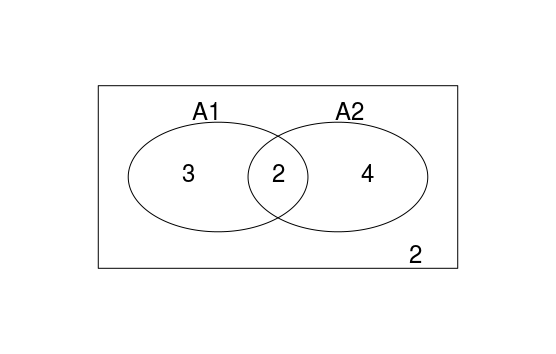
\includegraphics[width=7.72in]{img/venngram}

\textbf{證明:}

先考慮 \(A_1 \cup A_2\) 是什麼(拆分成三個互斥事件)

\(A_1 \cup A_2 = (A_1\cap \bar{A_2})\cup(\bar{A_1}\cap A_2)\cup(A_1\cap A_2)\)

運用上面的公理\sout{2} 3

\(\therefore P(A_1 \cup A_2) = P(A_1\cap \bar{A_2}) + P(\bar{A_1}\cap A_2) + P(A_1\cap A_2) \;\;\;\;\;\;(1)\)

再考慮 \(A_1=(A_1\cap A_2)\cup(A_1\cap\bar{A_2})\)
繼續拆分成兩個互斥事件

\(\therefore P(A_1)=P(A_1\cap A_2)+P(A_1\cap\bar{A_2})\) 整理一下:

\(P(A_1\cap\bar{A_2})=P(A_1)-P(A_1\cap A_2)\)

同理可得: \(P(\bar{A_1}\cap A_2)=P(A_2)-P(A_1\cap A_2)\)

代入上面第(1)式可得:

\(P(A_1 \cup A_2) =P(A_1)-P(A_1\cap A_2)\\ \;\;\;\;\;\;\;\;\;\;\;\;\;\;\;\;\;\;\;\;\;\;\;\;+P(A_2)-P(A_1\cap A_2)\\ \;\;\;\;\;\;\;\;\;\;\;\;\;\;\;\;\;\;\;\;\;\;\;\;+P(A_1\cap A_2)\\ \;\;\;\;\;\;\;\;\;\;\;\;\;\;\;\;\;\;=P(A_1) + P(A_2) - P(A_1 \cap A_2)\)

\section{條件概率 Conditional
probability}\label{-conditional-probability}

\begin{itemize}
\tightlist
\item
  \(P(A|S)=\frac{P(A\cap S)}{P(S)}\)
\item
  \(P(A\cap S) = P(A|S)P(S)\)
\end{itemize}

\section{獨立 (independence) 的定義}\label{-independence-}

\begin{itemize}
\tightlist
\item
  兩個事件定義爲互爲獨立時 (\(A\) and \(B\) are said to be independent
  \textbf{if and only if}) \[P(A\cap B)=P(A)P(B)\]
\item
  因爲從條件概率的概念我們已知 \(P(A\cap B) = P(A|B)P(B)\)
  所以\(P(A|B)=P(A)\) 即:事件 \(B\) 無法提供事件 \(A\) 的任何有效訊息
  (\textbf{\(A, B\) 互相獨立})
\end{itemize}

\section{賭博問題}

終於來到本次話題的``重點''了。

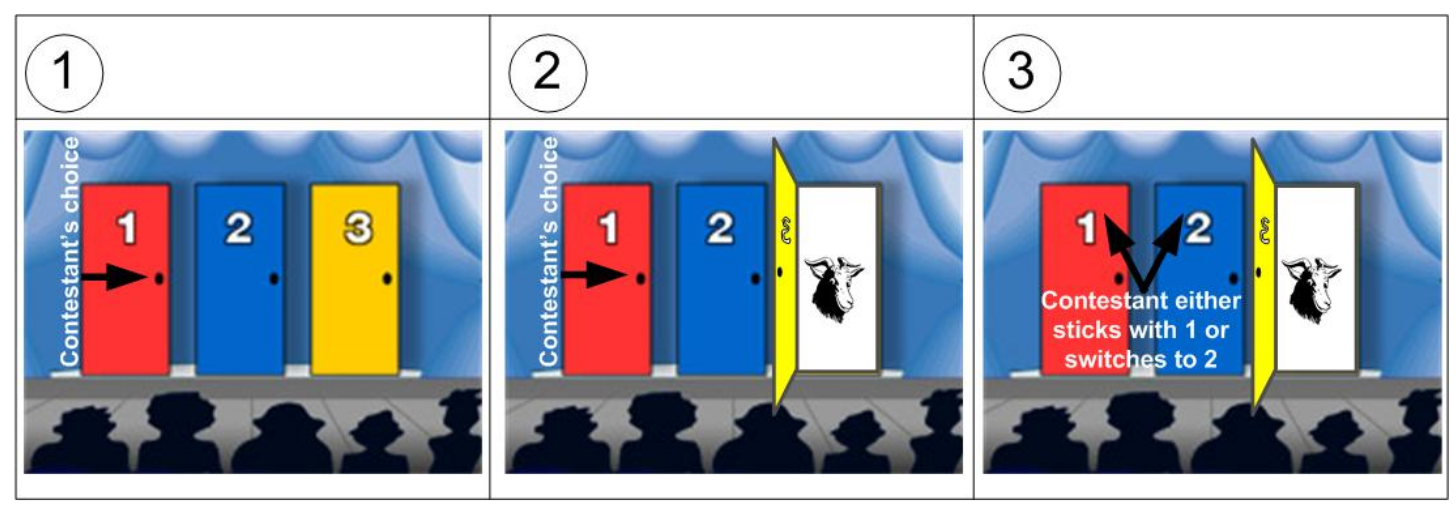
\includegraphics[width=20.22in]{img/Selection_071}

假設你在一個電視遊戲節目。有上圖一樣的三扇門。其中一扇門後面有一輛保時捷,另兩扇門後面則是\href{https://winterwang.github.io/post/black-meal/}{(味道奇特的)山羊}。遊戲規則是主持人會讓你先選擇其中一扇門(先不打開你選的這扇門)。主持人隨後打開另外兩扇門中的一扇沒有保時捷的門。主持人問你,你要堅持選擇之前選中的那扇門,還是要改變主意換一扇門去猜是否可以猜中保時捷。
請問,堅持選擇之前選中的門猜中保時捷的概率高,還是主持人打開一扇門以後改變主意猜中保時捷的概率更高呢?

\section{賭博問題的答案}

\textbf{答案是:必須改變主意才能提高中獎概率。}

上述情況下,最簡單的是用概率樹 (probability tree) 來做決定:

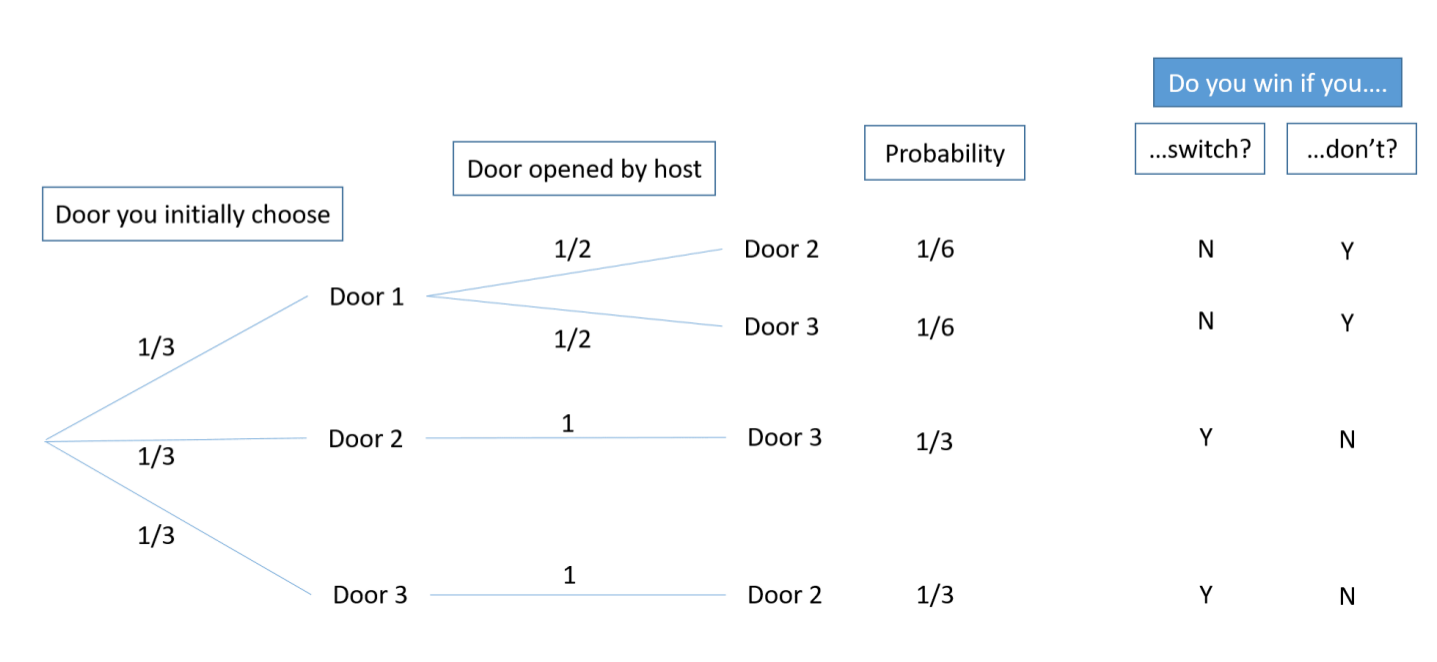
\includegraphics[width=19.96in]{img/Selection_072}

解說一下:

\begin{itemize}
\tightlist
\item
  假定保時捷在1號門後,你第一次選擇了1號門,那麼此時主持人可以任意打開2號或者三號門(因爲他們後面都沒有保時捷)。
\item
  假定保時捷在1號門後,你第一次選了2號門,那麼此時主持人只能打開3號門(因爲一號門後是保時捷,按照遊戲規則主持人不能打開)。
\item
  假定保時捷在1號門後,你第一次選了3號門,那麼此時主持人只能打開2號門(因爲一號門後是保時捷,按照遊戲規則主持人不能打開)。
\end{itemize}

所以按照圖中給出的計算概率樹的過程可以得到:

\[P[change]=\frac{1}{3}+\frac{1}{3}=\frac{2}{3}\\
P[not\; change]=\frac{1}{6}+\frac{1}{6}=\frac{1}{3}\]

你是否選擇了改變主意了呢?

\chapter{Bayes 貝葉斯理論的概念}\label{bayes-}

許多時候,我們需要將概率中的條件相互對調。 例如:
在已知該人羣中有20\%的人有吸菸習慣(\(P(S)\)),吸菸的人有9\%的概率有哮喘(\(P(A|S)\)),不吸菸的人有7\%的概率有哮喘(\(P(A|\bar{S})\))的前提下,有個人前來門診,發現是哮喘患者,那麼這個人有多大的概率是一個菸民?也就是要求
\(P(S|A)\)

這裏先引入貝葉斯的概念:

我們可以將 \(P(A\cap S)\) 寫成: \[P(A\cap S)=P(A|S)P(S)\\or\\
P(A\cap S)=P(S|A)P(A)\] 這兩個等式是完全等價的。我們將他們連起來:

\[P(S|A)P(A)=P(A|S)P(S)\\
\Rightarrow P(S|A)=\frac{P(A|S)P(S)}{P(A)}\]

是不是看起來又像是寫了一堆\textbf{廢話}?
沒錯,你看出來是一堆廢話的時候,證明你也同意這背後的簡單邏輯。

再繼續,我們可以利用另外一個\textbf{廢話}:\(\because S+\bar{S}=1\\ \therefore P(A)=P(A\cap S)+P(A\cap\bar{S})\)

用上面的公式替換掉
\(P(A\cap S)+P(A\cap\bar{S}) \\ \therefore P(A)=P(A|S)P(S)+P(A|\bar{S})P(\bar{S})\)

可以得到\textbf{貝葉斯理論公式}:

\[P(S|A)=\frac{P(A|S)P(S)}{P(A|S)P(S)+P(A|\bar{S})P(\bar{S})}\]

回到上面說到的哮喘人中有多少比例吸菸的問題。可以繼續使用概率樹來方便的計算:

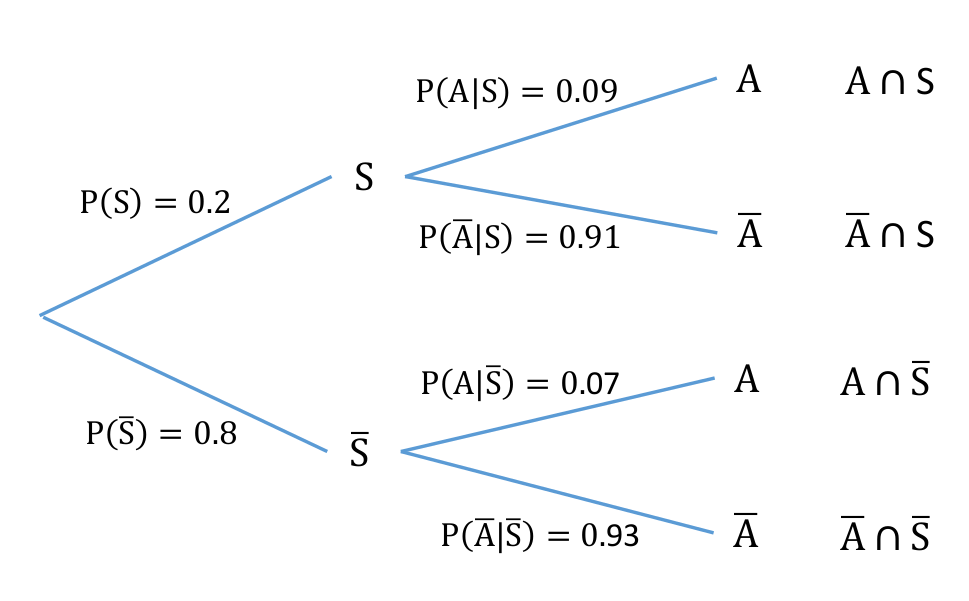
\includegraphics[width=13.46in]{img/Selection_073}

\begin{align}
P(S|A) &= \frac{P(A|S)P(S)}{P(A|S)P(S)+P(A|\bar{S})P(\bar{S})} \\
        &= \frac{0.09\times0.2}{0.09\times0.2+0.07\times0.8} \\
        &= 0.24
\end{align}

所以我們的結論就是,在已知該人羣中有20\%的人有吸菸習慣(\(P(S)\)),吸菸的人有9\%的概率有哮喘(\(P(A|S)\)),不吸菸的人有7\%的概率有哮喘(\(P(A|\bar{S})\))的前提下,有個人前來門診,發現是哮喘患者,那麼這個人有24\%
的概率是一個菸民(\(P(S|A)\))。

\chapter{期望 Expectation (或均值 or mean) 和 方差
Variance}\label{-expectation--or-mean---variance}

期望(或均值)是用來描述一組數據中心位置的指標(另一個是中位數
Median)。 對於離散型隨機變量 \(X\) (discrete random
variables),它的期望被定義爲:

\[E(X)=\sum_x xP(X=x)\]

所以就是將所有 \(X\)
可能取到的值乘以相應的概率後求和。這個期望(或均值)常常用希臘字母
\(\mu\) 來標記。

方差 Variance 是衡量一組數據變化幅度(dispersion/variability)的指標之一。
方差的定義是:

\[Var(X)=E((X-\mu)^2)\\其中,\mu=E(x)\]

實際上我們更加常用的是它的另外一個公式:

\[Var(X)=E(X^2)-E(X)^2\]

\textbf{證明 上面兩個方差公式相等}

\begin{align}
Var(x)  &= E((X-\mu)^2) \\
        &= E(X^2-2X\mu+\mu^2)\\
        &= E(X^2) - 2\mu E(X) + \mu^2\\
        &= E(X^2) - 2\mu^2 + \mu^2 \\
        &= E(X^2) - \mu^2 \\
        &= E(X^2) - E(X)^2
\end{align}

\section{方差的性質:}

\begin{enumerate}
\def\labelenumi{\arabic{enumi}.}
\tightlist
\item
  \(Var(X+b)=Var(X)\)
\item
  \(Var(aX)=a^2Var(X)\)
\item
  \(Var(aX+b)=a^2Var(X)\)
\end{enumerate}

\chapter{伯努利分佈 Bernoulli
distribution}\label{-bernoulli-distribution}

伯努利分佈,說的就是一個簡單的二分變量 (1, 0),它取1時的概率如果是
\(\pi\)。那麼我們可以計算這個分佈的期望值:

\begin{align}
E(X) &=\sum_x xP(X=x) \\
     &=1\times\pi + 0\times(1-\pi)\\
     &=\pi
\end{align}

由於 \(x=x^2\),因爲 \(x=0,1\), 所以 \(E[X^2]=E[X]\),那麼方差爲:

\begin{align}
Var(X) &=E[X^2]-E[X]^2 \\
       &=E[X]-E[X]^2 \\
       &=\pi - \pi^2 \\
       &=\pi(1-\pi)
\end{align}

\textbf{證明,\(X,Y\) 爲互爲獨立的隨機離散變量時,a) \(E(XY)=E(X)E(Y)\)
; b) \(Var(X+Y)=Var(X)+Var(Y)\)}

\begin{itemize}
\item
  \begin{enumerate}
  \def\labelenumi{\alph{enumi})}
  \tightlist
  \item
    \textbf{證明}
  \end{enumerate}
\end{itemize}

\begin{align}
E(XY) &= \sum_x\sum_y xyP(X=x, Y=y) \\
\because &\; X,Y are\;independent\;to\;each\;other \\
\therefore &= \sum_x\sum_y xyP(X=x)P(Y=y)\\
      &=\sum_x xP(X=x)\sum_y yP(Y=y)\\
      &=E(X)E(Y)
\end{align}

\begin{itemize}
\item
  \begin{enumerate}
  \def\labelenumi{\alph{enumi})}
  \setcounter{enumi}{1}
  \tightlist
  \item
    \textbf{證明} 根據方差的定義:

    \begin{align}
    Var(X+Y) &= E((X+Y)^2)-E(X+Y)^2 \\
     & \; Expand \\
     &=E(X^2+2XY+Y^2)-(E(X)+E(Y))^2\\
     &=E(X^2)+E(Y^2)+2E(XY)\\
     &\;\;\; - E(X)^2-E(Y)^2-2E(X)E(Y)\\
     &\; We\;just\;showed\; E(XY)=E(X)E(Y)\\
     &=E(X^2)-E(X)^2+E(Y^2)-E(Y)^2 \\
     &=Var(X)+Var(Y)
    \end{align}
  \end{enumerate}
\end{itemize}

\chapter{二項分佈的概念 Binomial
distribution}\label{-binomial-distribution}

二項分佈在醫學研究中至關重要,一組二項分佈的數據,指的通常是 \(n\)
次相互獨立的\href{https://winterwang.github.io/post/probability2-4/}{成功率爲
\(\pi\) 的伯努利實驗} (\(n\) independent Bernoulli trials)
中成功的次數。

當 \(X\) 服從二項分佈,記爲 \(X \sim binomial(n, \pi)\)
或\(X \sim bin(n, \pi)\)。它的(第 \(x\) 次實驗的)概率被定義爲:

\begin{align}
P(X=x) &= ^nC_x\pi^x(1-\pi)^{n-x} \\
       &= \binom{n}{x}\pi^x(1-\pi)^{n-x} \\
       & for\;\; x = 0,1,2,\dots,n
\end{align}

\section{二項分佈的期望和方差}

\begin{itemize}
\tightlist
\item
  期望 \(E(X)\)

  \begin{itemize}
  \tightlist
  \item
    若 \(X \sim bin(n,\pi)\),那麼 \(X\)
    就是這一系列獨立伯努利實驗中成功的次數。
  \item
    用 \(X_i, i =1,\dots, n\) 標記每個相互獨立的伯努利實驗。
  \item
    那麼我們可以知道 \(X=\sum_{i=1}^nX_i\)。

    \begin{align} E(X) &= E(\sum_{i=1}^nX_i)\\
                     &= E(X_1+X_2+\cdots+X_n) \\
                     &= E(X_1)+E(X_2)+\cdots+E(X_n)\\
                     &= \sum_{i=1}^nE(X_i)\\
                     &= \sum_{i=1}^n\pi \\
                     &= n\pi
      \end{align}
  \end{itemize}
\item
  方差 \(Var(X)\)

  \begin{align}
  Var(X) &= Var(\sum_{i=1}^nX_i) \\
      &= Var(X_i+X_2+\cdots+X_n) \\
      &= Var(X_i)+Var(X_2)+\cdots+Var(X_n) \\
      &= \sum_{i=1}^nVar(X_i) \\
      &= n\pi(1-\pi) \\
  \end{align}
\end{itemize}

\section{超幾何分佈 hypergeometric
distribution}\label{-hypergeometric-distribution}

假設我們從總人數爲 \(N\) 的人羣中,採集一個樣本
\(n\)。假如已知在總體人羣中(\(N\))有 \(M\)
人患有某種疾病。請問採集的樣本 \(X=n\)
中患有這種疾病的人,服從怎樣的分佈?

\begin{itemize}
\tightlist
\item
  從人羣(\(N\))中取出樣本(\(n\)),有 \(^NC_n\) 種方法。
\item
  從患病人羣(\(M\))中取出患有該病的人(\(x\))有 \(^MC_x\) 種方法。
\item
  樣本中不患病的人(\(n-x\))被採樣的方法有 \(^{N-M}C_{n-x}\) 種。
\item
  採集一次 \(n\) 人作爲樣本的概率都一樣。因此:
\end{itemize}

\[P(X=x)=\frac{\binom{M}{x}\binom{N-M}{n-x}}{\binom{N}{n}}\]

\section{樂透中獎概率問題:}

\begin{itemize}
\tightlist
\item
  從數字 \(1\sim59\) 中選取 \(6\) 個任意號碼
\item
  開獎時從 \(59\) 個號碼球中隨機抽取 \(6\) 個
\item
  如果六個號碼全部猜中(不分順序),你可以成爲百萬富翁。請問一次猜中全部
  \(6\) 個號碼的概率是多少?
\end{itemize}

從 \(59\) 個號碼中隨機取出任意 \(6\) 個號碼的方法有 \(^{59}C_6\) 種。
\[^{59}C_6=\frac{59!}{6!(59-6)!}=45,057,474\]

每次選取六個號碼做爲一組的可能性相同,所以,你買了一組樂透號碼,能中獎的概率就是
\(1/45,057,474 = 0.00000002219\)。你還會再去買彩票麼?

\subsection{\texorpdfstring{如果我只想中其中的 \(3\)
個號碼,概率有多大?}{如果我只想中其中的 3 個號碼,概率有多大?}}\label{-3-}

用超幾何分佈的概率公式:

\begin{align}
P(X=3) &= \frac{^6C_3\times ^{53}C_3}{^{59}C_6} \\
       &= 0.010
\end{align}

你有 \(1\%\)
的可能中獎。換句話說,如果中三個以上的數字算中獎的話,你買的彩票中獎的概率低於
\(1\%\)。是不是覺得下次送錢給博彩公司的時候還不如跟我一起喝一杯咖啡划算?

\chapter{泊松分佈 Poisson Distribution}\label{-poisson-distribution}

\begin{itemize}
\tightlist
\item
  當一個事件,在一段時間 (\(T\)) 中可能發生的次數是 \(\lambda\)
  。那麼我們可以認爲,經過時間 \(T\),該時間發生的期望次數是
  \(E(X)=\lambda T\)。
\item
  利用微分思想,將這段時間 \(T\) 等分成 \(n\) 個時間段,當
  \(n\rightarrow\infty\) 直到每個微小的時間段內最多發生一次該事件。
\end{itemize}

那麼

\begin{itemize}
\tightlist
\item
  每個微小的時間段,可以視爲是一個伯努利實驗(有事件發生或者沒有)
\item
  那麼這整段時間 \(T\) 內發生的事件可以視爲是一個二項分佈實驗。
\end{itemize}

令 \(X=\) 一次事件發生時所經過的所有時間段。

\begin{itemize}
\tightlist
\item
  \(X \sim Bin(n, \pi)\),其中 \(n\rightarrow\infty\),\(n\) 爲時間段。
\item
  在每個分割好的時間段內,事件發生的概率都是:\(\pi=\frac{\lambda T}{n}\)
\item
  期望 \(\mu=\lambda T \Rightarrow \pi=\mu/n\)
\item
  所以 \(X\) 的概率方程就是:

  \begin{align}
  P(X=x) &= \binom{n}{x}\pi^x(1-\pi)^{n-x} \\
     &= \binom{n}{x}(\frac{\mu}{n})^x(1-\frac{\mu}{n})^{n-x} \\
     &= \frac{n!}{x!(n-x)!}(\frac{\mu}{n})^x(1-\frac{\mu}{n})^{n-x} \\
     &=\frac{n!}{n^x(n-x)!}\frac{\mu^x}{x!}(1-\frac{\mu}{n})^{n-x}\\
  when\; n\rightarrow\infty   &\; x \ll n\\
  \frac{n!}{n^x(n-x)!} &=\frac{n(n-1)\dots(n-x+1)}{n^x} \rightarrow 1\\
  (1-\frac{\mu}{n})^{n-x} &\approx  (1-\frac{\mu}{n})^n \rightarrow e^{-\mu}\\
  the\;probability\;function&\;of\;a\;Poisson\;distribution   \\
  P(X=x) &\rightarrow \frac{\mu^x}{x!}e^{-\mu}
  \end{align}
\end{itemize}

當數據服從泊松分佈時,記爲
\(X\sim Poisson(\mu=\lambda T)\;\; or\;\; X\sim Poi(\mu)\)

\textbf{證明泊松分佈的參數特徵:}

\begin{enumerate}
\def\labelenumi{\arabic{enumi}.}
\tightlist
\item
  \(E(X)=\mu\)
\end{enumerate}

\begin{align}
E(X)  &=  \sum_{x=0}^\infty xP(X=x) \\
      &=  \sum_{x=0}^\infty x\frac{\mu^x}{x!}e^{-\mu} \\
      &= 0+ \sum_{x=1}^\infty x\frac{\mu^x}{x!}e^{-\mu} \\
      &=  \sum_{x=1}^\infty \frac{\mu^x}{(x-1)!}e^{-\mu} \\
      &=  \mu\sum_{x=1}^\infty \frac{\mu^{x-1}}{(x-1)!}e^{-\mu} \\
replace\; &x\; with\; all\; i=x-1 \\
      &=  \mu\sum_{i=0}^\infty \frac{\mu^{i}}{i!}e^{-\mu} \\
notice\; that\; &the\; right\; side \sum_{i=0}^\infty \frac{\mu^{i}}{i!}e^{-\mu}=1 is \\
the\;sum\;of\;all\;&probability\;of\;a\;Poisson\;distribution\\
      &= \mu
\end{align}

\begin{enumerate}
\def\labelenumi{\arabic{enumi}.}
\setcounter{enumi}{1}
\tightlist
\item
  \(Var(x)=\mu\) 爲了找到 \(Var(X)\),我們用公式
  \(Var(X)=E(X^2)-E(X)^2\)
\end{enumerate}

我們需要找到 \(E(X^2)\)

\begin{align}
E(X^2) &= \sum_{x=0}^\infty x^2\frac{\mu^x}{x!}e^{-\mu} \\
       &= \mu \sum_{x=1}^\infty x\frac{\mu^{x-1}}{(x-1)!}e^{-\mu} \\
replace\; &x\; with\; all\; i=x-1 \\
       &= \mu \sum_{i=0}^\infty (i+1)\frac{\mu^{i}}{i!}e^{-\mu} \\
       &= \mu(\sum_{i=0}^\infty i\frac{\mu^i}{i!}e^{-\mu} + \sum_{i=0}^\infty \frac{\mu^i}{i!}e^{-\mu}) \\
       &= \mu(E(X)+1) \\
       &= \mu^2+\mu \\
Var(X) &= E(X^2) - E(X)^2 \\
       &= \mu^2 + \mu -\mu^2 \\
       &= \mu
\end{align}

\chapter{正態分佈}

\section{概率密度曲線 probability density function,
PDF}\label{-probability-density-function-pdf}

\begin{itemize}
\item
  一個隨機連續型變量 \(X\) 它的性質由一個對應的\textbf{概率密度方程
  (probability density function, PDF)} 決定。
\item
  在給定的範圍區間內,如 \(a\sim b, (a < b)\),它的概率滿足:
\end{itemize}

\[P(a\leqslant X \leqslant b) = \int_a^bf(x)dx\]

\begin{itemize}
\tightlist
\item
  這個相關的方程,在 \(a\sim b\)
  區間內的積分,就是這個連續變量在這個區間內取值的概率。
\end{itemize}

\begin{Shaded}
\begin{Highlighting}[]
\CommentTok{# R codes for drawing a standard normal distribution by using ggplot2}
\KeywordTok{library}\NormalTok{(ggplot2)}
\NormalTok{p <-}\StringTok{ }\KeywordTok{ggplot}\NormalTok{(}\KeywordTok{data.frame}\NormalTok{(}\DataTypeTok{x=}\KeywordTok{c}\NormalTok{(}\OperatorTok{-}\DecValTok{3}\NormalTok{,}\DecValTok{3}\NormalTok{)), }\KeywordTok{aes}\NormalTok{(}\DataTypeTok{x=}\NormalTok{x)) }\OperatorTok{+}
\StringTok{  }\KeywordTok{stat_function}\NormalTok{(}\DataTypeTok{fun =}\NormalTok{ dnorm)}
\NormalTok{p }\OperatorTok{+}\StringTok{ }\KeywordTok{annotate}\NormalTok{(}\StringTok{"text"}\NormalTok{, }\DataTypeTok{x=}\DecValTok{2}\NormalTok{, }\DataTypeTok{y=}\FloatTok{0.3}\NormalTok{, }\DataTypeTok{parse=}\OtherTok{TRUE}\NormalTok{, }\DataTypeTok{label=}\StringTok{"frac(1, sqrt(2*pi)) * e ^(-z^2/2)"}\NormalTok{) }\OperatorTok{+}
\StringTok{  }\KeywordTok{theme}\NormalTok{(}\DataTypeTok{plot.subtitle =} \KeywordTok{element_text}\NormalTok{(}\DataTypeTok{vjust =} \DecValTok{1}\NormalTok{),}
        \DataTypeTok{plot.caption =} \KeywordTok{element_text}\NormalTok{(}\DataTypeTok{vjust =} \DecValTok{1}\NormalTok{),}
        \DataTypeTok{axis.text.x =} \KeywordTok{element_text}\NormalTok{(}\DataTypeTok{size =} \DecValTok{12}\NormalTok{),}
        \DataTypeTok{axis.text.y =} \KeywordTok{element_text}\NormalTok{(}\DataTypeTok{size =} \DecValTok{12}\NormalTok{),}
        \DataTypeTok{plot.title =} \KeywordTok{element_text}\NormalTok{(}\DataTypeTok{size =} \DecValTok{10}\NormalTok{, }\DataTypeTok{face =} \StringTok{"bold"}\NormalTok{, }\DataTypeTok{hjust =} \FloatTok{0.5}\NormalTok{),}
        \DataTypeTok{panel.background =} \KeywordTok{element_rect}\NormalTok{(}\DataTypeTok{fill =} \StringTok{"ivory"}\NormalTok{)) }\OperatorTok{+}
\StringTok{  }\KeywordTok{labs}\NormalTok{(}\DataTypeTok{title =} \StringTok{"Probability density functions }\CharTok{\textbackslash{}n}\StringTok{ for standard normal distribution"}\NormalTok{,}
       \DataTypeTok{x =} \OtherTok{NULL}\NormalTok{, }\DataTypeTok{y =} \OtherTok{NULL}\NormalTok{) }\OperatorTok{+}
\StringTok{  }\KeywordTok{stat_function}\NormalTok{(}\DataTypeTok{fun =}\NormalTok{ dnorm,}
                \DataTypeTok{xlim =} \KeywordTok{c}\NormalTok{(}\OperatorTok{-}\FloatTok{1.3}\NormalTok{,}\FloatTok{0.4}\NormalTok{),}
                \DataTypeTok{geom =} \StringTok{"area"}\NormalTok{,}\DataTypeTok{fill=}\StringTok{"#00688B"}\NormalTok{, }\DataTypeTok{alpha=} \FloatTok{0.2}\NormalTok{)}
\end{Highlighting}
\end{Shaded}

\begin{figure}

{\centering 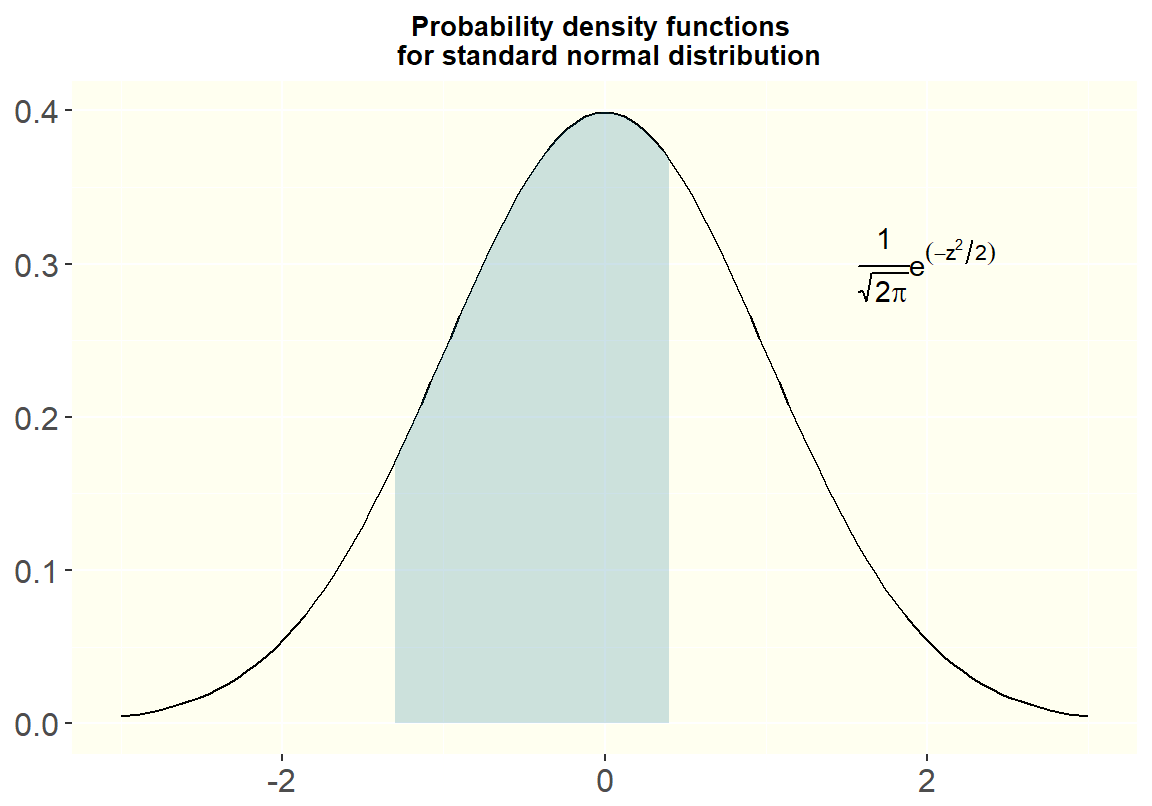
\includegraphics[width=0.9\linewidth]{bookdown_files/figure-latex/PDF-standard-1} 

}

\caption{Probability Density Function of a Standard Normal Distribution}\label{fig:PDF-standard}
\end{figure}

注意:整個方程的曲線下面積等於 \(1\):
\[\int_{-\infty}^\infty f(x)dx=1\]

\begin{itemize}
\tightlist
\item
  期望 \(E(X)=\int_{-\infty}^\infty xf(x)dx\)
\item
  方差 \(Var(X)=\int_{-\infty}^\infty (x-\mu)^2f(x)dx\)
\end{itemize}

\section{正態分佈}\label{-1}

如果一組數據服從正態分佈,我們通常用它的期望(或者叫平均值)\(\mu\),和它的方差
\(\sigma^2\),來描述這組數據。記爲:

\[X \sim N(\mu, \sigma^2)\]

\begin{itemize}
\tightlist
\item
  它的概率密度方程可以表述爲:
\end{itemize}

\[f(x)=\frac{1}{\sqrt{2\pi\sigma^2}}exp(-\frac{(x-\mu)^2}{2\sigma^2})\]

\begin{itemize}
\tightlist
\item
  \(E(x) =\mu\)
\item
  \(Var(x)=\sigma^2\)
\end{itemize}

\section{標準正態分佈}

標準正態分佈的期望(或者均值)爲 \(0\),方差爲 \(1\)

\begin{itemize}
\tightlist
\item
  記爲:\(Z \sim N(0,1)\)
\item
  它的概率密度方程表述爲:
\end{itemize}

\[\frac{1}{\sqrt{2\pi}}exp(-\frac{z^2}{2})\]

\begin{itemize}
\tightlist
\item
  它的累積分佈方程 (cumulative distribution function,
  CDF),是將概率密度方程 (PDF) 積分以後獲得的方程。通常我們記爲
  \(\Phi(z)\)
\end{itemize}

再看一下標準正態分佈的概率密度方程曲線:

\begin{figure}

{\centering 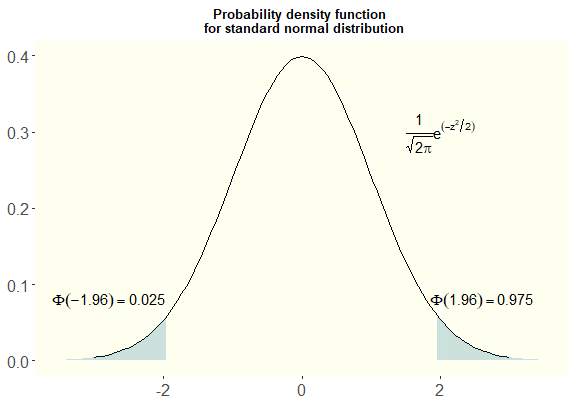
\includegraphics[width=0.9\linewidth]{bookdown_files/figure-latex/PDF-standard2-1} 

}

\caption{Probability Density function of a Standard Normal Distribution}\label{fig:PDF-standard2}
\end{figure}

\begin{itemize}
\tightlist
\item
  95\% 的曲線下面積在標準差 standard deviation \(-1.96\sim1.96\)
  之間的區域。
\item
  而且,\(\phi(-x)=1-\phi(x)\)
\item
  任何一個正態分佈都可以通過下面的公式,標準化成爲標準正態分佈:
\end{itemize}

\[Z=\frac{X-\mu}{\sigma}\]

\chapter{中心極限定理 the Central Limit
Theorem}\label{-the-central-limit-theorem}

最近明顯可以感覺到課程的步驟開始加速。看我的課表:

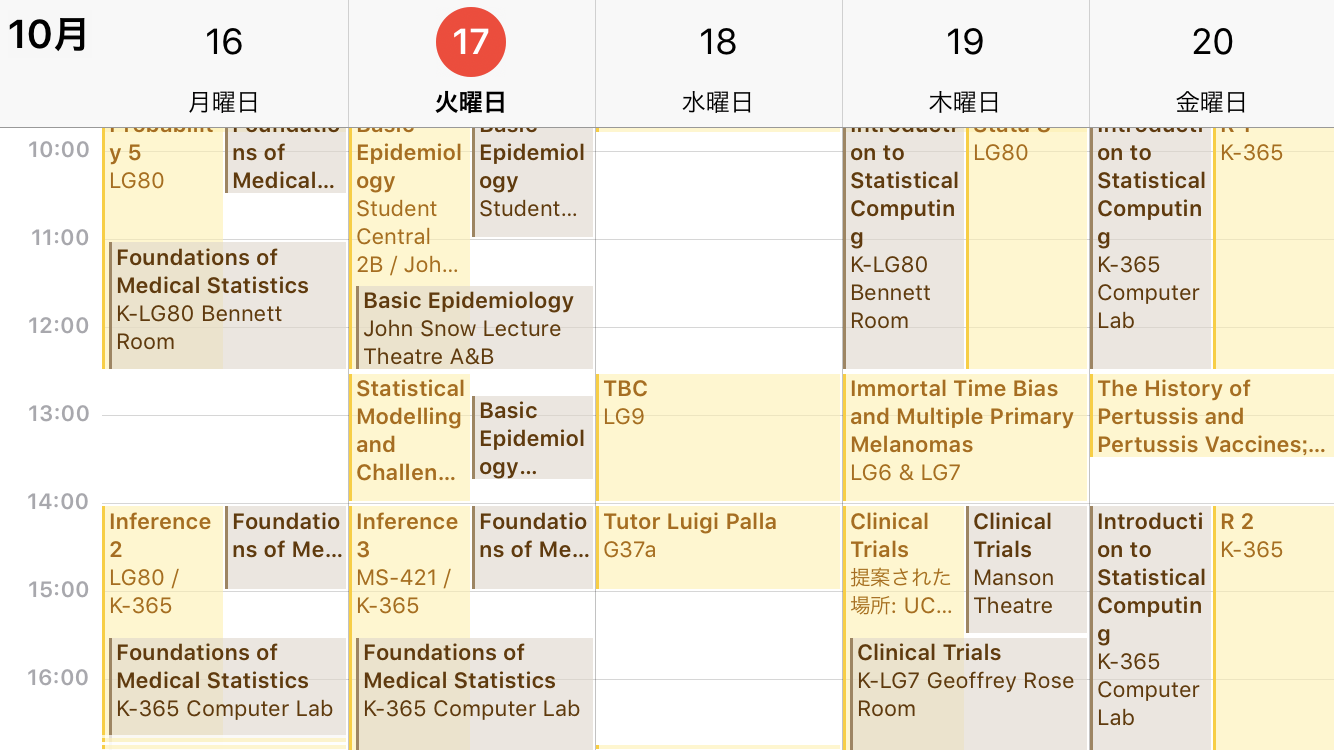
\includegraphics[width=18.53in]{img/IMG_0522}

手機畫面太小了。早上都是9點半開始,下午基本都是到5點。週一更慘,到7點。週二-週五中午都被統計中心的講座佔據。簡直是非人的生活。

這周概率論基礎結束。中心極限定理講完以後我們正式進入了 Inference
統計推斷的課程。我們花了一天時間講什麼是樣本估計
(Estimation),什麼是參數精確度 (Precision),什麼是自由度 (degree of
freedom),怎樣進行不偏的估計 (unbiased inference)。然後還有似然方程
(likelihood function)。

今天的更新還是簡單的把概率論掃尾一下。感受一下中心極限定理的偉大。

\section{協方差 Covariance}\label{-covariance}

\href{https://winterwang.github.io/post/probability2-4/}{之前我們定義過},兩個獨立連續隨機變量
\(X,Y\) 之和的方差 Variance :

\[Var(X+Y)=Var(X)+Var(Y)\]

然而如果他們並不相互獨立的話:

\begin{aligned}
Var(X+Y) &= E[((X+Y)-E(X+Y))^2] \\
         &= E[(X+Y)-(E(X)+E(Y))^2] \\
         &= E[(X-E(X)) - (Y-E(Y))^2] \\
         &= E[(X-E(X))^2+(Y-E(Y))^2 \\
         & \;\;\; +2(X-E(X))(Y-E(Y))] \\
         &= Var(X)+Var(Y)+2E[(X-E(X))(Y-E(Y))]
\end{aligned}

可以發現在兩者和的方差公式展開之後多了一部分 \(E[(X-E(X))(Y-E(Y))]\)。
這個多出來的一部分就說明了二者 \((X, Y)\) 之間的關係。它被定義爲協方差
(Covariance): \[Cov(X,Y) = E[(X-E(X))(Y-E(Y))]\]

所以:

\[Var(X+Y)=Var(X)+Var(Y)+2Cov(X,Y)\]

要記住,協方差只能用於評價\(X,Y\)之間的線性關係 (Linear Association)。

以下是協方差 (Covariance) 的一些特殊性質:

\begin{enumerate}
\def\labelenumi{\arabic{enumi}.}
\tightlist
\item
  \(Cov(X,X)=Var(X)\)
\item
  \(Cov(X,Y)=Cov(Y,X)\)
\item
  \(Cov(aX,bY)=ab\:Cov(X,Y)\)
\item
  \(Cov(aR+bS,cX+dY)=ac\:Cov(R,X)+ad\:Cov(R,Y)\\ \;\;\;\;\;\;\;\;\;\;\;\;\;\;\;\;\;\;\;\;\;\;\;\;\;\;\;\;\;\;\;\;\;\;\;\;\;+bc\:Cov(S,X)+bd\:Cov(S,Y)\)
\item
  \(Cov(aX+bY,cX+dY)=ac\:Var(X)+ad\:Var(Y)\\ \;\;\;\;\;\;\;\;\;\;\;\;\;\;\;\;\;\;\;\;\;\;\;\;\;\;\;\;\;\;\;\;\;\;\;\;\;+(ad+bc)Cov(X,Y)\)
\item
  \(Cov(X+Y,X-Y)=Var(X)-Var(Y)\)
\item
  If \(X, Y\) are independent. \(Cov(X,Y)=0\) {But not vise-versa !}
\end{enumerate}

\section{相關 Correlation}\label{-correlation}

\begin{itemize}
\tightlist
\item
  協方差雖然\(Cov(X,Y)\)
  的大小很大程度上會被他們各自的單位和波動大小左右。
\item
  我們將協方差標準化(除以各自的標準差 s.d.) (standardization)
  之後,就可以得到相關係數 Corr (\(-1\sim1\)):
  \[Corr(X,Y)=\frac{Cov(X,Y)}{SD(X)SD(Y)}=\frac{Cov(X,Y)}{\sqrt{Var(X)Var(Y)}}\]
\end{itemize}

\section{中心極限定理 the Central Limit
Theorem}\label{-the-central-limit-theorem-1}

\textbf{如果從人羣中多次選出樣本量爲 \(n\) 的樣本,並計算樣本均值,
\(\bar{X}_n\)。那麼這個樣本均值 \(\bar{X}_n\) 的分佈,會隨着樣本量增加
\(n\rightarrow\infty\),而接近正態分佈。}

偉大的中心極限定理告訴我們:

\textbf{當樣本量足夠大時,樣本均值 \(\bar{X}_n\)
的分佈爲正態分佈,這個特性與樣本來自的人羣的分佈 \(X_i\) 無關。}

\textbf{再說一遍:}

如果對象是獨立同分佈 i.i.d (identically and independently
distributed)。那麼它的總體期望和方差分別是:
\(E(X)=\mu;\;Var(X)=\sigma^2\)。 根據中心極限定理,可以得到:

\begin{itemize}
\tightlist
\item
  當樣本量增加,樣本均值的分佈服從正態分佈:
  \[\bar{X}_n\sim N(\mu, \frac{\sigma^2}{n})\]
\item
  也可以寫作,當樣本量增加: \[\sum_{i=1}^nX_i \sim N(n\mu,n\sigma^2)\]
\item
  有了這個定理,我們可以拋開樣本空間(\(X\))的分佈,也不用假定它服從正態分佈。
\item
  但是樣本的均值,卻總是服從正態分佈的。簡直是太完美了!!!!!!
\end{itemize}

\part{統計推斷 Inference}\label{part--inference}

\chapter{統計推斷的概念}

\subsection{人羣與樣本 (population and
sample)}\label{-population-and-sample}

討論樣本時,需考慮下面幾個問題:

\begin{enumerate}
\def\labelenumi{\arabic{enumi}.}
\tightlist
\item
  樣本是否具有代表性?
\item
  人羣被準確定義了嗎?
\item
  我們感興趣的``人羣''是否可以是無限大(多)的?
\item
  我們研究的樣本,是僅僅用來觀察,亦或是計劃對之進行某種干預呢?
\item
  我們從所有可能的人羣中抽樣了嗎?
\end{enumerate}

\subsection{樣本和統計量 (sample and
statistic)}\label{-sample-and-statistic}

通常我們在進行實驗或觀察時只是獲得了樣本的數據。而希望從樣本數據去推斷
(inference)
總體(或人羣)的一些特徵。我們也許只是想用樣本的平均值來估計整體人羣的某個特徵的平均值。不管是何種估計和推斷,都是基於對樣本數據的計算,從樣本中獲得想要推斷總體的\textbf{統計量
(statistics)}。我們用已知樣本去推斷未知總體的過程就叫做\textbf{估計
(estimate)}。這個想要被推斷的總體或人羣的值,被叫做\textbf{參數
(parameter)},常常使用希臘字母來標記。用來估計總體或人羣的,從樣本數據計算得來的統計量,叫做\textbf{估計量
(estimator)}。

所有的統計量,都有\textbf{樣本分佈 (sampling
distributions,意爲重複無限次取樣後獲得的無限次統計量的分佈)}。推斷的過程歸納如下:

\begin{enumerate}
\def\labelenumi{\arabic{enumi}.}
\tightlist
\item
  從總體或人羣中抽樣 (樣本量 \(n\))
\item
  計算這個樣本的合適統計量,從而用於估計它在整體或人羣中的值。
\item
  我們還需要決定計算獲得的統計量的樣本分佈(假定會抽樣無數次)。
\item
  一旦可以精確地確認樣本分佈,我們就可以定量地計算出使用步驟2中獲得的統計量估計總體或人羣的參數時的準確度。
\end{enumerate}

\subsection{估計 Estimation}\label{-estimation}

從樣本的均值,推斷總體或人羣的均值是一種估計。我們的目的是,從已知樣本中計算一個儘可能接近那個未知的總體或人羣參數的值。一個估計量有兩個與生俱來的性質
(properties):1) 偏倚 (bias); 2) 精確度
(precision)。這兩個性質都可以從樣本分佈和估計量獲得。

\begin{enumerate}
\def\labelenumi{\arabic{enumi}.}
\item
  偏倚:
  偏倚簡單說就是樣本分佈的均值,也就是我們從樣本中計算獲得的估計量,和我們想要拿它來估計的總體或人羣的參數之間的差距。(The
  bias is the difference between the mean of the sampling distribution
  -- the expected or average value of the estimator -- and the
  population parameter being estimated.)
  一個小的偏倚,確保了我們從樣本中計算獲得的估計值(假設我們抽樣無數次,計算無數個樣本估計值)\textbf{均勻地}分佈在總體或人羣參數的左右兩邊。偏倚本身並不是太大的問題,但是假如樣本量增加,偏倚依然存在(估計量不一致,
  inconsistent),那常常意味着是抽樣過程出現了問題。例如:用簡單隨機抽樣法獲得的樣本均值,就是總體或人羣均值的無偏估計
  (unbiased
  estimator)。如果抽樣時由於某些主觀客觀的原因導致較小的樣本很少被抽樣(抽樣過程出了問題,脫離了簡單隨機抽樣原則),那麼此時得到的樣本均值就會是一個過高的估計值
  (upward biased estimator)。
\item
  精確度:估計值的精確度可以通過樣本分佈的方差或標準差來評價(簡單說是樣本分佈的方差越低,波動越小,精確度越高)。樣本分佈的標準差被定義爲估計值的標準誤。假如估計量是樣本均值,那麼樣本分佈的標準差(估計量的標準誤)和樣本數據之間有如下的關係:
  \[均值的標準誤 = \frac{樣本數據的標準差}{\sqrt{樣本量大小}}\]
\end{enumerate}

在一些簡單的情況下,通常估計值的選用不言自明(例如均值,或者百分比)。但是在複雜的情況下,我們可能可以有多個不同類型的估計量可以選擇,他們也常常各有利弊,需要我們做出取捨。

\subsection{信賴區間 confidence intervals}\label{-confidence-intervals}

從樣本中計算估計量獲得的一個估計值,只是一個\textbf{點估計 (point
estimate)}。對比之下,信賴區間就是一個對這個點估計的精確度的體現。信賴區間越窄,說明我們對於總體或人羣的參數的可能取值的範圍估計越精確。

信賴區間通常是成對成對的出現的,即有上限和下限。這樣的一對從樣本數據中計算得來的統計量,同樣也是有樣本分佈的。\textbf{每次我們重新從總體或人羣中抽樣,計算獲得的信賴區間都不同,這些信賴區間就組成了信賴區間的樣本分佈。總體和人羣的參數落在這些信賴區間範圍內的概率,就是我們常說的信賴區間的水平(\(95\%\))。}
常用的這個概率值就是 \(95\%, 90\%, 99\%\)。

當從樣本數據計算獲得的估計量的信賴區間很寬,說明了這個收集來的數據提供了很少的參數信息,導致估計變得很不精確。

\emph{看到這裏的都是好漢一條啊!
我不知道你暈了麼有,反正我是已經暈了。。。。}

\part{統計分析方法 Analytical
Techniques}\label{part--analytical-techniques}

\chapter{探索數據和簡單描述}

\part{貝葉斯統計}\label{part-}

\chapter{貝葉斯統計入門}

\part{臨床實驗 Clinical Trials}\label{part--clinical-trials}

\chapter{臨床實驗原則}

\bibliography{book.bib,packages.bib}

\backmatter
\printindex

\end{document}
